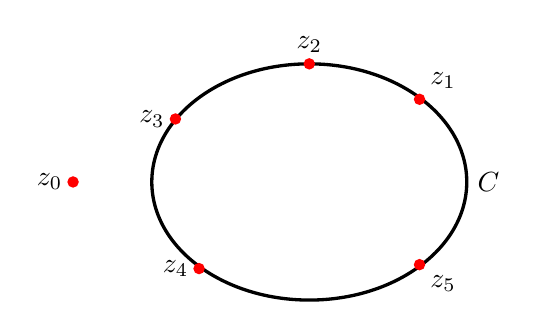
\begin{tikzpicture}[very thick]
  \draw (0,0) ellipse (2 and 1.5) (2,0) node [right] {$C$};
  \draw[red,fill] (-3, 0) circle (0.05) node [black, left] {$z_0$};
  \draw[red, fill] (1.4, 1.05) circle (0.05) node [black, above right] {$z_1$}
  (0,1.5) circle (0.05) node [black, above] {$z_2$}
  (-1.7,.8) circle (0.05) node [black, left] {$z_3$}
  (-1.4,-1.1) circle (0.05) node [black, left] {$z_4$}
  (1.4,-1.05) circle (0.05) node [black, below right] {$z_5$};
\end{tikzpicture}

%%% Local Variables:
%%% mode: latex
%%% TeX-master: "../main"
%%% End:
